%
% (File) acl2018.tex
%
%% Based on the style files for ACL-2017, with some changes, which were, in turn,
%% Based on the style files for ACL-2015, with some improvements
%%  taken from the NAACL-2016 style
%% Based on the style files for ACL-2014, which were, in turn,
%% based on ACL-2013, ACL-2012, ACL-2011, ACL-2010, ACL-IJCNLP-2009,
%% EACL-2009, IJCNLP-2008...
%% Based on the style files for EACL 2006 by
%%e.agirre@ehu.es or Sergi.Balari@uab.es
%% and that of ACL 08 by Joakim Nivre and Noah Smith

\documentclass[11pt,a4paper]{article}
\usepackage[hyperref]{acl2018}
\usepackage{times}
\usepackage{latexsym}

\usepackage{color}

\usepackage{amsmath,amsthm}
\theoremstyle{definition}
\newtheorem*{defn}{Definition}

\usepackage[ruled]{algorithm2e}

\usepackage{graphicx}
\usepackage{epstopdf}


\usepackage{url}

%\aclfinalcopy % Uncomment this line for the final submission
%\def\aclpaperid{***} %  Enter the acl Paper ID here


%\setlength\titlebox{5cm}
% You can expand the titlebox if you need extra space
% to show all the authors. Please do not make the titlebox
% smaller than 5cm (the original size); we will check this
% in the camera-ready version and ask you to change it back.
\newcommand{\secref}[1]{Section \ref{#1}}
\newcommand{\figref}[1]{Figure \ref{#1}}
\newcommand{\eqnref}[1]{Eq. (\ref{#1})}
\newcommand{\exref}[1]{Example \ref{#1}}
\newcommand{\algoref}[1]{Algorithm \ref{#1}}
\newcommand{\tabref}[1]{Table \ref{#1}}
\newcommand{\socvec}{SocVec}
\newcommand{\argmin}{\operatornamewithlimits{argmin}}
\newcommand{\argmax}{\operatornamewithlimits{argmax}}
\newtheorem{example}{Example}
\newtheorem{lemma}{Lemma}
\newtheorem{definition}{Definition}
\newcommand{\cut}[1]{}

\newcommand\BibTeX{B{\sc ib}\TeX}
\newcommand{\KZ}[1]{\textcolor{red}{Kenny: #1}}
\newcommand{\KQ}[1]{\textcolor{blue}{Kangqi: #1}}
\newcommand{\YY}[1]{\textcolor{orange}{Yangyang: #1}}

\title{Triple Construction Algorithms for Joint Extraction of Entities and Relations}

\author{First Author \\
  Affiliation / Address line 1 \\
  Affiliation / Address line 2 \\
  Affiliation / Address line 3 \\
  {\tt email@domain} \\\And
  Second Author \\
  Affiliation / Address line 1 \\
  Affiliation / Address line 2 \\
  Affiliation / Address line 3 \\
  {\tt email@domain} \\}

\date{}

\begin{document}
\maketitle
\begin{abstract}
Previously a novel tagging scheme was proposed to jointly
extract entities and relations at the same time and showed
good results. In this process, relation triples must be
eventually recovered from the predicted sequence of special tags.
Previous algorithm to construct the triples was simple and naive.
This paper presents a few new triple construction algorithms
that results in substantial improvement on the end-to-end
relation extraction task.
\end{abstract}


\section{Introduction}
\label{sec:intro}

Evaluation of dialogue systems is an open question. Existing
automatic evaluation metrics for chitchat systems are similar to those for 
other text generation tasks (e.g., machine translation \citep{papineni-etal-2002-bleu}, question-answering \citep{rajpurkar-etal-2016-squad}, 
summarization \citep{lin-2004-rouge}), which depends on calculating word overlaps with 
ground truth reference responses. 
However, for chitchat tasks, there are usually 
many alternative but plausible responses given a situation, 
perhaps more than any other text generation task mentioned above. 
A limited number of reference responses are 
not sufficient to determine how good a generated response is. 
Moreover, such static settings are not good at
assessing an interactive, context-sensitive system.

Interactive human evaluation metrics usually 
involve a Likert scale evaluation after a multi-turn conversation 
with the evaluated bot. 
While this method is a step up from the previous static evaluation, 
it is difficult for human judges to give a concrete score to
any bot.
%\KZ{But are we also asking judges to score invidividual bots, which is difficult?} 
To compare the performance of two bots is easier. 
Thus ACUTE-EVAL~\citep{DBLP:journals/corr/abs-1909-03087} asks the 
judges to make a binary judgment of who is better in conversations between two identical bots 
or between a human and a bot. A more advanced version of that
is \textit{Spot The Bot}~\cite{deriu-etal-2020-spot} which models the 
human evaluation of a 
conversation after the Turing test. Such a process is still 
time-consuming and costly, 
compared with automatic evaluations.

In our opinion, a good method for evaluating multi-turn conversational model/system 
should satisfy the following requirements:
i) be as efficient and inexpensive as possible;
ii) can truly reflect a model's ability to conduct a human conversation; 
iii) evaluation results should correlate well with human judgments;
iv) can be used to compare and rank the capabilities of a set of models/systems.
  
Toward that goal, in this work, we propose an automatic interactive evaluation framework, 
which is called \textit{ChatMatch} for chitchat
agents. This framework can be used to rank any number of bots with very little
time and effort.  Above all, we want to emphasize the significance of
the observation on direct interactions between bots in the evaluation. 
People tend to believe that human-bot conversations are more reliable 
and produce more comprehensive evaluations of chatbots' capabilities. 
This is not always true. As human annotators know their counterpart is a robot, 
they tend to ask common and goal-directed questions. 
The bot-bot chat logs in our experiments show that, surprisingly,  
talking between two different bots may expose both their strengths and weaknesses not seen
in human-bot conversations. 
Here, we take as an example in \figref{fig:two convs} two small fragments 
from the chat logs between humans-bot and bot-bot. While talking about hobbies, 
human keeps asking the bot direct questions, which leads to boring responses from the bot.
However, in a bot-bot setting, two bots, including the same bot in the previous
conversation, start explaining their hobbies to each other, producing a much more natural and 
interesting conversation. 

\begin{figure}[ht!]
\begin{subfigure}{0.5\textwidth}
  \centering
  % include first image
  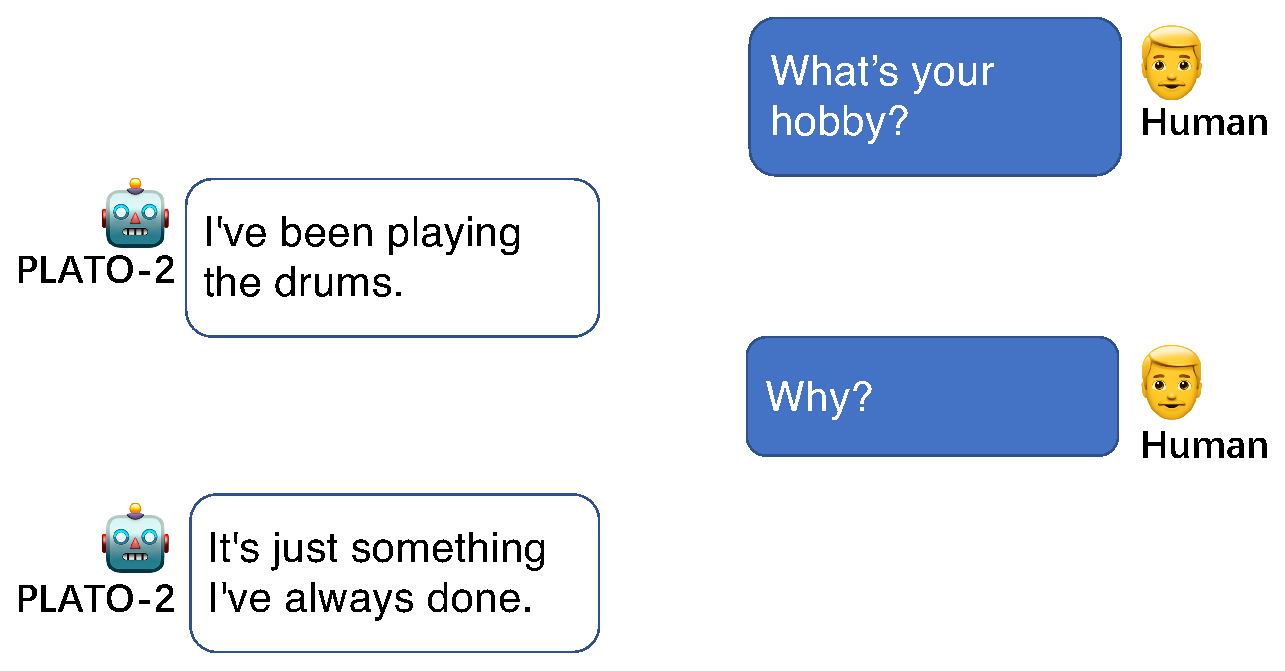
\includegraphics[width=.8\linewidth]{crop1.eps}  
  \caption{A small fragment of conversation between human and bot}
  \label{fig:sub-first}
\end{subfigure}
\begin{subfigure}{0.5\textwidth}
  \centering
  % include second image
  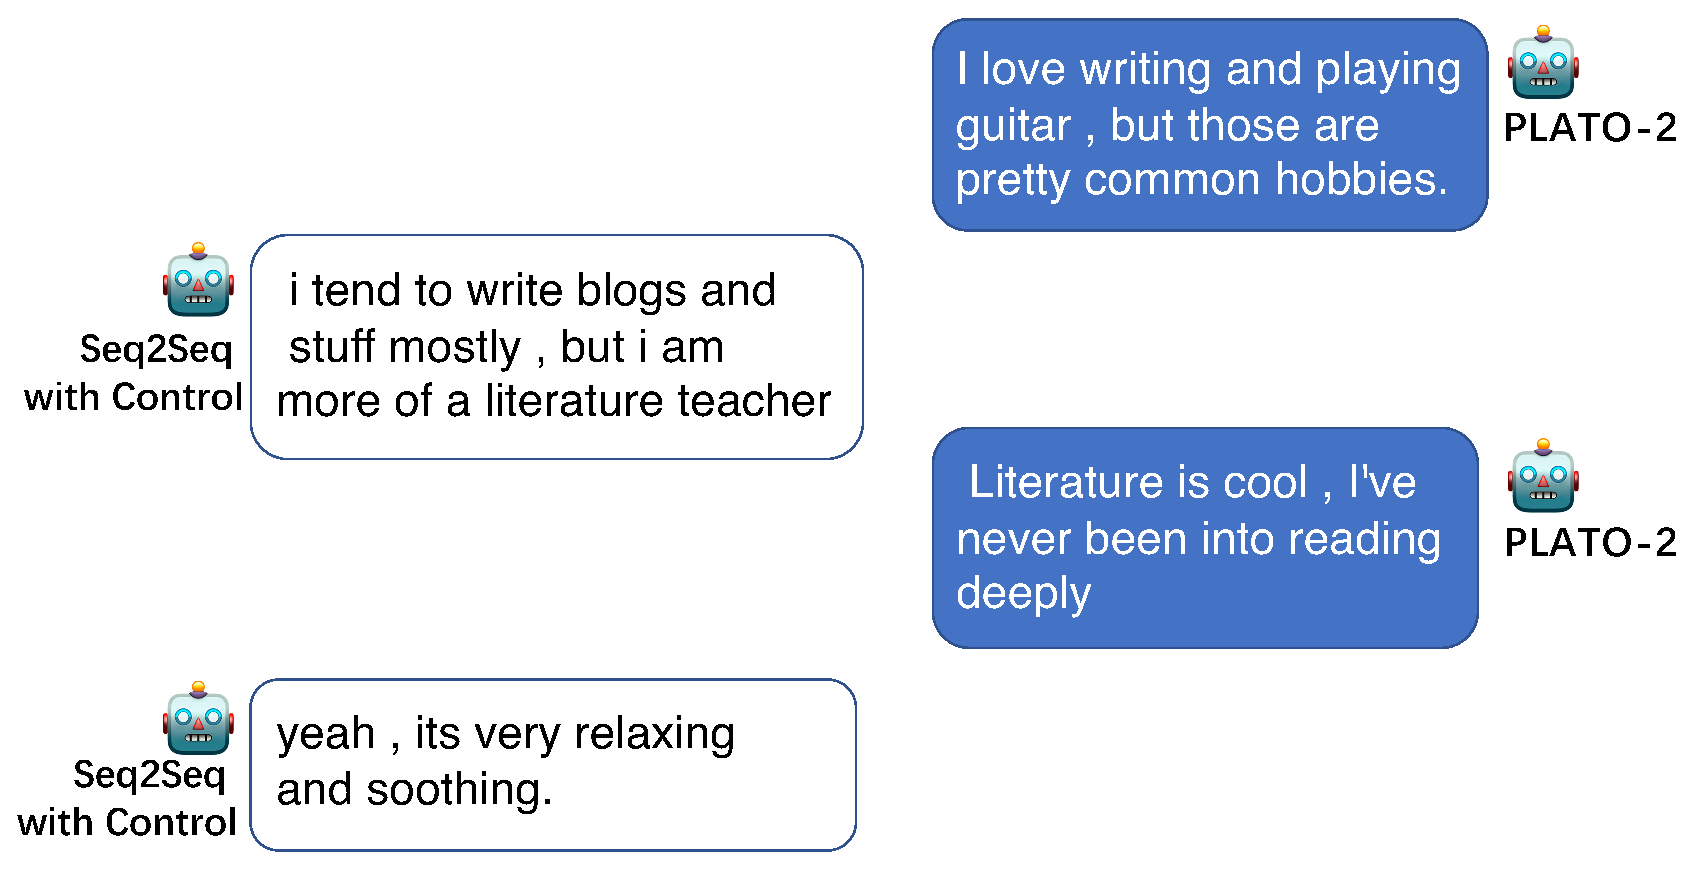
\includegraphics[width=\linewidth]{crop2.eps}  
  \caption{A small fragment of conversation between bot and bot% \KZ{crop the margins
%in this pic or use eps for both.} 
}
  \label{fig:sub-second}
\end{subfigure}
\caption{Small fragments from the chat logs between humans-bot and bot-bot}
\label{fig:two convs}
\end{figure}

Our framework consists of two components: \textit{competition} and 
\textit{scoring}, which may happen simultaneously. The competition is modeled
after most sport tournaments such as soccer or ping pong. 
There are three levels of competitions: 
game-level, match-level and tournament-level. 
Each match consists of several games. During a game, two bots will converse 
freely with each other and a virtual judge will score their performances according to
a group of criteria such as consistency and fluency, etc. 
%As an example like \figref{fig:example} shows, 
%Bot $A$ will be 
%penalized twice for repeating while Bot $B$ will be penalized once for 
%contradicting itself. In addition to the penalty, 
%a bonus point is rewarded to $A$
%who shows to produce relevant response with long term memory. 
%\KZ{Do we still have this as a criterion?}
%However, the specific bonus and penalty settings may vary 
%depending on the domain and scenarios that the experiment is 
%set in. 

%\begin{figure}[th!]
%	\centering
%	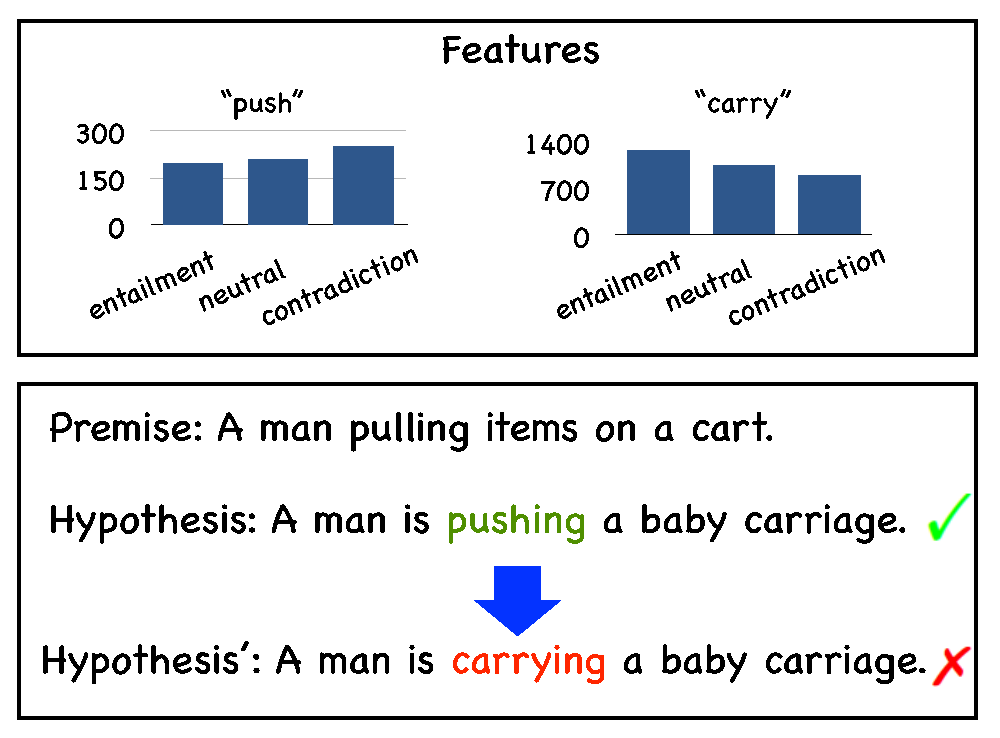
\includegraphics[width=0.95\columnwidth]{example.eps}
%	\caption{A chat snippet between two bots.}
%	\label{fig:example}
%\end{figure}

The main contributions of this paper are:
\begin{itemize}
\item We propose the first interactive evaluation framework for chatbots which
is based solely on bot-to-bot conversations and modeled after sports competitions (\secref{sec:competition}).
\item  The entire scoring process is fully automated and efficient. 
The system can rank seven bots in three minutes on average.
(\secref{sec:scoring}, \secref{sec:time}).
\item  Our experiments show that our scoring system closely tracks the 
human evaluation results. Preliminary results also show
that our evaluation system outperforms 
several recent strong baseline evaluation systems (\secref{sec:main}).
\item %We demonstrate the improvements in efficiency 
%using direct chat logs between bots.
We show that the chats between bots are impressively informative, 
even richer than the chats between humans and bots.
This suggests some possible directions to improve 
the capabilities of bots in the future.
(e.g., by having them learn from each other)  (\secref{sec:diversity})
\end{itemize}

%\section{Problem Definition}
\label{sec:problem}

In this section we formally define the problem of short title extraction.
A char is a single Chinese or English character.
A segmented word (or term) $x$ is a sequence of several chars such as 
``Nike'' or ``牛仔裤''(jean).
A product title, denoted as $X$, is a sequence of words $\{x_1, x_2, ..., x_n\}$.
Let $Y$ be a sequence of labels $\{y_1, y_2, ..., y_n\}$ over $X$, where $y_i \in \{0, 1\}$.
The corresponding short title is a subsequence of $X$, denoted as $S = \{x_i\}$, 
where $y_i = 1$ and $|S| \le n$.

%we are interesting in obtaining a short title which can represent the most important information about the product.

We regard short title extraction task as a sequence classification problem.
Each word is sequentially visited in the original product title order
and a binary decision is made.
We do this by scoring each word $x_i$ within $X$ and predicting a label $y_i \in \{0, 1\}$, 
indicating whether the word should or should not be included in the short title $S$.
As we apply supervised training, the objective is to maximize the likelihood of all word labels
$Y=\{y_1,y_2,...,y_n\}$, given the input product title $X$ and model parameters $\theta$:
\begin{equation}
\label{eqn:problem}
\log{p(Y|X,\theta)}=\sum_{i=1}^{n}{\log{p(y_i|X,\theta)}}.
\end{equation}

%Our problem is different from Sequece Labelling problem, as ...

%In a more restrictive scenario, the number of words $m$ in the short title is strictly limited, where $m$ is some fixed number and $m \le \sum_{i=1}^{n} len(x_i)$. $len(x_i)$ is the number of words (chars) in term $x_i$.


%\section{Sentiment-Aspect-Region Model}
\label{sec:model}
We first present our objectives to build the
unified sentiment-aspect-region model.
To achieve the objectives, we present several intuitions
based on which we build our model.
We then describe the details of the model,
and propose a parameter estimation method.

\subsection{Intuitions}
\label{sec:motiv}
%We first introduce some notions that are used in
%explaining our objectives. There are three types of
%latent factors that are not observable in a geotagged review corpus, but
%are important for user preference analysis. They
%are topical-region, topical-aspect and sentiment.
%A topical-region represents a geographical area in which
%users do similar things (such as dining).
%%write region-specific words on their reviews.
%It comprises two components: geo-location and semantics.
%The geo-location component is usually modeled as a
%Gaussian distribution over
%POIs \cite{Yin:2011,YuanW4:2013}.
%The semantic component is modeled as a multinomial
%distribution over words \cite{Geofolk:2010}.
%Example topical-regions include shopping areas, education areas,
%streets of special snacks, etc.
%Topical-aspects are the aspects of POIs that
%are commented by users, such as environment, taste,
%price, etc. Sentiments are user's opinions over
%topical-aspects (e.g., positive, negative or neutral).
%%\KZ{Can sentiments be casted over regions? e.g., I hate
%%Clarke Quay!}
%Topical-aspects
%and sentiments can be modeled jointly \cite{JoASUM:2011}.

In this paper,
we aim at building a model that is able to 1) extract
latent variables, i.e., topical-aspect, sentiment,
and topical-region from the review
data; 2) capture the interdependencies among
category, POI, user, words and the three latent
variables; and 3) discover user's topical-region and
topical-aspect preferences.
To achieve these objectives,
we exploit the following intuitions in designing our model:

\textbf{Intuition 1}: A user visits POIs in a topical-region
because the region is geographically convenient to the user
(e.g., close to her activity areas) and its topics (e.g., shopping
street, education area, etc.) satisfy
the user's interest. Each user has her own preferences on the
topical-regions.
%We use a topical-region
%variable $r$ to model the mixture of topic and geographic
%information,
%i.e., each region exactly covers POIs of similar
%topic distribution and close in spatial.

\textbf{Intuition 2}: A user rates highly of a POI because
she likes some aspects of the POI. Such preferences might be
indicated in her review.
%i.e., user has preferences on some aspects of the POI.
Some users like to check the price range of a restaurant first while
others might be more concerned with the environment. Moreover, POIs in different
categories may have different aspects of interest.
%For
%instance, a traveler might care more about the environment
%of a hotel, while a hungry would-be diner might be more interested in
%the waiting time of a restaurant.

\textbf{Intuition 3}:
A user decides to visit a POI in a region
by considering the category, category-aware topical-aspects of the POI and
the distance to it. For example, users may visit POIs of the
restaurant category with good environment,
but she may first consider the restaurants nearby.
%to walk around a nearby shopping street.
%and visit
%POIs without being particular about the category.

\textbf{Intuition 4}: When a user writes a review on a POI, she
will use words for both the aspects of the POI and
her sentiments about the aspects.
The user may also use words for the topical-region of the POI.
For example, a review on a shop in Times Square may say:
``This shop offers best prices in Times Square.'' The reviewer
uses ``price'' for {\em aspect}, ``best'' for {\em sentiment}
and ``Times Square'' for {\em region}. %to construct the review.
%Moreover, each sentence in the review normally
%corresponds to exactly one aspect and
%users only associate one sentiment on each aspect. As a result,
%the words co-occurs in the same sentences are more likely to be correlated to
%the same aspect and sentiment.

\subsection{Model Description}
We first define the notations
to be used in the proposed model. Let $D$ be the set of user reviews,
and $U$ be the set of users. For each review, we denote the
number of its sentences by $M$ and number of words in each
sentence by $N$. In our model, a location has two attributes:
identifier and coordinates. We use $l$ to represent a location identifier
and $\boldsymbol{cd}_l$ to denote its corresponding coordinates.
Here $\boldsymbol{cd}_l$ is a latitude and longitude pair. We denote
the topical-aspect, sentiment and topical-region by $a$, $s$,
and $r$, respectively. The notations
used in this paper are listed in \tabref{tab:notation}.
Following the intuitions discussed in \secref{sec:motiv}, we
proceed to present our model.

\begin{table}[th]
\centering
%\scriptsize
\caption{Description of Symbols}
\begin{tabular}{l|l}
\hline
 Symbol & Description\\
\hline
$u$, $U$ & individual user and the set of users\\
\hline
$l$, $L$ & individual POI and the set of POIs  \\
\hline
$c$ & category  \\
\hline
$r$ & topical-region  \\
\hline
$a$, $s$ & topical-aspect and sentiment \\
\hline
$d$, $D$ & single review and the set of reviews \\
\hline
$M$ & the number of sentences in a review \\
\hline
$w$, $N$ & single word and the number of words in a sentence \\
\hline
\end{tabular}
\label{tab:notation}
\end{table}

Based on \textbf{Intuitions 1\&2}, we model the user
topical-region preferences and topical-aspect preferences
as multinomial distributions $p(r|u)$ and $p(a|u,c)$, respectively.

Based on \textbf{Intuition 3}, a user chooses a POI to visit
by considering both the category and the distance. We
define the probability of visiting a POI $l$ given
category $c$ and region $r$ proportional to $p(l|c)\cdot p(l|r)$.
Here $p(l|c)$ is the probability of selecting POI $l$ from
the category $c$; $p(l|r)$ is a the probability
of selecting POI $l$ in region $r$ by considering
the distance from $l$ to $r$. After normalization, we have the
definition $p(l|c,r)=\frac{p(l|c)p(l|r)}{\sum_{l'}{p(l'|c)p(l'|r)}}$.
%The denominator is used to normalize
%the $p(l|c)p(l|r)$ over all POIs.
To model the spatial distance, we use a
Gaussian mixture model, i.e.,
$p(l|r)\sim N(\boldsymbol{\mu}_r, \boldsymbol{\Sigma}_r)$, where
$\boldsymbol{\mu}_r$ is the center of region $r$ and
$\boldsymbol{\Sigma}_r$ is the co-variance matrix which depicts the
area of region $r$.
To model the membership of a POI to a category, we use a uniform
distribution for $p(l|c)$.
%$\kappa$ is tunable parameter used
%for balance the weights of generating POI from category and region.
%Note that $p(l|r)$ is a continuous distribution while $p(l|c)$ is
%a discrete distribution.
%To multiply the two distributions,
%we adopt the coordinate transformation approach for the Gaussian
%distribution that is proposed in Yuan et al.\cite{YuanW4:2013}.

Based on \textbf{Intuition 4},
we model the relationships among words, topical-aspects,
sentiments and topical-regions by
$p(w|a,s,r)=\lambda p(w|a,s)+(1-\lambda) p(w|r)$, where
$a$, $s$, $r$ are topical-aspect, sentiment and
topical-region, respectively.
Here $p(w|a,s)$ is the probability that the users write
word $w$ when they have sentiment $s$ on aspect $a$;
$p(w|r)$ is the probability that the users use word
$w$ to describe region $r$; parameter
$\lambda$ is used to balance the portion of
words drawn from topical-aspect, sentiment or topical-region.
We model $p(w|a,s)$ instead of $p(w|a)$ and $p(w|s)$
because aspects and sentiments are closely coupled,
and modeling by $p(w|a)$ and $p(w|s)$
needs an additional tuning parameter.
Similar to proposals of sentence level sentiment analysis
\cite{TitovMGLDA:2008,TitovMAS:2008, JoASUM:2011},
we assume each sentence expresses opinions on exactly one topical-aspect
and each topical-aspect is associated to a positive, negative or neutral sentiment.

\begin{figure}[th]
\centering
\epsfig{file=fig/modeldraft.eps,width=0.65\columnwidth}
\caption{Sentiment-Aspect-Region Model (SAR)}
\label{fig:model}
\end{figure}

In summary, the graphical representation of our model
is shown in \figref{fig:model} and
the generative process of the
reviews written by user $u$ is described as follows:
\begin{itemize}
\item For each review $d\in D_u$, where $D_u$ is the set of reviews written by user $u$.
    \begin{itemize}
    \item Draw topical region $r\sim p(r|u)$
    \item Draw category $c\sim p(c|u)$
    \item Draw location $l\sim p(l|c,r)=\frac{p(l|r)p(l|c)}{\sum_{l'}{p(l'|c)p(l'|r)}}$, where $p(l|r)\sim N(\boldsymbol{\mu}_r,\boldsymbol{\Sigma}_r)$
    \item For each sentence in review $d$
        \begin{itemize}
        \item Draw aspect $a\sim p(a|u,c)$
        \item Draw sentiment $s\sim p(s|a,l)$
        \item For each word position in the sentence
            \begin{itemize}
            \item Draw word $w\sim p(w|a,s,r)={\lambda}p(w|a,s)+(1-\lambda)p(w|r)$
            \end{itemize}
        \end{itemize}
    \end{itemize}
\end{itemize}

In the model, $p(l|c)$ and
$p(c|u)$ can be estimated directly from a given corpus. The
other distribution parameters need to be inferred.
We first present how to estimate $p(l|c)$ and
$p(c|u)$, and then show the inference algorithm for
the remaining distributions in \secref{sec:infer}.

As described in \textbf{Intuition 3},
a POI $l$ is generated from both category
and region. Since POI $l$ and category $c$ are
observable variables, we simply compute $p(l|c)$
by \equref{eq:plc}.
\begin{equation}
p(l|c)=\frac{I(l,c)}{\#\; of\; POIs\; in\; c}
\label{eq:plc}
\end{equation}
\begin{equation}
I(l,c)=
\begin{cases}
1 & l\in c \\
0 & otherwise \\
\end{cases}
\end{equation}

Similarly, we compute the category preferences of each user, i.e., $p(c|u)$,
directly from the corpus. To handle the overfitting problem,
we apply the additive smoothing technique. After smoothing, even though a user did
not a visit some category of POIs, the probability of
visiting that category still has a small value. The computation of $p(c|u)$ is shown in
\equref{eq:pcu}.
\begin{equation}
p(c|u)=\frac{n_c+\alpha}{N+{\alpha}C},
\label{eq:pcu}
\end{equation}
where $n_c$ is the number of reviews of POIs in category $c$ that user $u$
writes; $N$ is the total number of reviews on POIs in $c$; $C$
is the total number of categories; $\alpha$  is the smoothing
parameter which is usually set to a value smaller than 1. In this paper,
we set $\alpha=0.1$.

\subsection{Inference Algorithm}
\label{sec:infer}
To infer the parameters of the model, we
use the expectation-maximization (EM) approach.
In this section,
we present the computation of the corpus
likelihood, the two-step EM algorithm
used to infer our parameters, and
initialization of the EM algorithm.

\subsubsection{Likelihood Computation}
Our model has several levels, i.e., word level,
sentence level, and document level. The latent variables
are on two levels. Region $r$ is at document level while
aspect $a$ and sentiment $s$ are at sentence level.
This multi-level structure poses challenges to the estimation of
the log-likelihood. According to the generative
process, we have the likelihood of the corpus $D$:
\begin{equation}
p(D;\Phi)=\prod_{d}^{D}{p(u_d)\sum_{r}^{R}{p(r|u_d)}p(l_d,\mathbf{w}_d|r,u_d)}
\label{eq:likeli1}
\end{equation}
\begin{equation}
p(l_d,\mathbf{w}_d|r,u_d)=p(c_{l_d}|u_d)p(l_d|r,c_{l_d})\prod_{i}^{M}{p(\mathbf{w}_{d,i}|c_{l_d},r,u_d,l_d)}
\label{eq:likeli2}
\end{equation}
\begin{equation}
\begin{split}
&p(\mathbf{w}_{d,i}|c_{l_d},r,u_d,l_d) \\
&=\sum_{a,s}{p(a|c_{l_d},u_d)p(s|a,l_d)\prod_{j}^{N}{p(w_{d,i,j}|a,s,r)}}
\end{split}
\label{eq:likeli3}
\end{equation}
In \equref{eq:likeli1}, $\Phi$ is the set of parameters in the model,
i.e., $p(r|u)$, $p(a|c,u)$,$p(l|r)$,$p(s|a,l)$,$p(w|a,s)$,
$p(w|r)$,$\boldsymbol{\mu}_r$ and $\boldsymbol{\Sigma}_r$.
Variables $u_d$,$l_d$,$\mathbf{w}_d$ are the user, location and
words of review $d$, respectively. Variable $\mathbf{w}_{d,i}$
represents the set of words in sentence $i$ of review $d$
while $w_{d,i,j}$ is the $j^{th}$ word in sentence
$i$ of review $d$. Taking logarithm of
$p(D;\Phi)$ leads to a summation inside the logarithm:
\begin{equation}
L=\sum_{d}{\log{p(u_d)}+\log{\sum_{r}{p(r|u_d)p(l_d,\mathbf{w}_d|r,u_d)}}}
\label{eq:loglikeli}
\end{equation}
Since this likelihood cannot be estimated directly,
we adopt Jessen's
inequality to the log-likelihood, and estimate the
lower bound of the likelihood and the parameters
in an iterative manner.

\subsubsection{Expectation-Maximization}
Due to the aforementioned difficulty of computing
log-likelihood directly,
we apply Expectation-Maximization (EM)
algorithm to estimate the model parameters.

In \textbf{E-step}, we compute the expectation
of latent variables given the observed data.
By applying Jessen's inequality to \equref{eq:loglikeli},
we get the lower bound of the likelihood as:
\begin{equation}
\begin{split}
L_{LB}=&\sum_{d}{\log{p(u_d)}}\\
+&\sum_{d,r}{p(r|d)(\log{p(r|u_d)}+\log{p(l_d,\mathbf{w}_d|r,u_d)})}
\end{split}
\label{eq:loglikeli1}
\end{equation}
As shown in \equref{eq:loglikeli1},
we need to estimate $p(r|d)$ to compute the full likelihood.
We apply Bayes rule, and obtain the update
function of the posterior distribution as
\begin{equation}
p(r|d)=\frac{p(r,d)}{\sum_{r}{p(r,d)}}
\label{eq:prd}
\end{equation}
\begin{equation}
p(r,d)=p(u_d)p(r|u_d)p(l_d,\mathbf{w}_d|r,u_d)
\label{eq:prdjoint}
\end{equation}
In \equref{eq:prdjoint},
$p(l_d,\mathbf{w}_d|r,u_d)$ is computed by \equref{eq:likeli2}, and
$p(u_d)$ appears both in the numerator and the denominator,
and thus is not necessary to estimate.

In \textbf{M-step}, by maximizing the lower bound of likelihood,
we can obtain the update function of parameters at document level
that are related to topical region $r$ as below.
\begin{equation}
p(r|u)=\frac{\sum_{d\in D_u}{p(r|d)}}{\sum_{r}{\sum_{d\in D_u}{p(r|d)}}}
\label{eq:pru}
\end{equation}
%\begin{equation}
%\boldsymbol{\mu}_r=\frac{\sum_{d}{p(r|d)\cdot \boldsymbol{cd}_{l_d}}}{\sum_{d}{p(r|d)}}
%\label{eq:mu}
%\end{equation}
%\begin{equation}
%\boldsymbol{\Sigma}_r=\frac{\sum_{d}{p(r|d)\cdot (\boldsymbol{cd}_{l_d}-\boldsymbol{\mu}_r)^T(\boldsymbol{cd}_{l_d}-\boldsymbol{\mu}_r)}}{\sum_{d}{p(r|d)}}
%\label{eq:sigma}
%\end{equation}

However, we cannot obtain a close form solution for $\boldsymbol{\mu}_r$ and
$\boldsymbol{\Sigma}_r$ due to the normalization term. We adopt a gradient method
to obtain the update value of $\boldsymbol{\mu}_r$ and $\boldsymbol{\Sigma}_r$ in M-step.
Specifically, we use the BFGS quasi-Newton method \cite{Kurashima:2013,Liu:1989}.
In the gradient method, we compute the gradient of $\boldsymbol{\mu}_r$ and
$\boldsymbol{\Sigma}_r$ as follows:
\begin{equation}
\frac{\partial L_{LB}}{\partial \boldsymbol{\mu}_r}=
\sum_d{p(r|d)\boldsymbol{\Sigma}_r^{-1}\left(\frac{\sum_{l'}{q(l')(\boldsymbol{cd}_{l'}-\boldsymbol{\mu}_r)}}{\sum_{l'}{q(l')}}-
(\boldsymbol{cd}_{l_d}-\boldsymbol{\mu}_r)\right)}
\label{eq:gmu}
\end{equation}
\begin{equation}
\frac{\partial L_{LB}}{\partial \boldsymbol{\Sigma}_r}=\sum_d{p(r|d)(\frac{\sum_{l'}{q(l')g(l', r)}}{\sum_{l'}{q(l')}}-g(l_d, r))}
\label{eq:gsigma},
\end{equation}
%\begin{equation}
%g(l, r)=-\frac{1}{2}\boldsymbol{\Sigma}_r^{-1}+\frac{1}{2}\boldsymbol{\Sigma}_r^{-1}(\boldsymbol{cd}_{l}-\mu_r)(\boldsymbol{cd}_{l}-\mu_r)^T\boldsymbol{\Sigma}_r^{-1}
%\end{equation}
where $q(l')=p(l'|c_l)p(l'|r)$ and $\boldsymbol{cd}_{l}$ denotes the coordinates of POI $l$.
The function $g(l, r)$ in \equref{eq:gsigma} is the gradient of the Gaussian distribution for region $r$
w.r.t. $\boldsymbol{\Sigma}_r$ at point $l$.

Since sentiment and aspect are at the sentence level, we
cannot compute $\log p(l_d,\mathbf{w}_d|r,u_d)$
in \equref{eq:loglikeli1} using $p(r|d)$. 
Thus, we propose a second level of EM iterations.
Specifically, we introduce a new latent variable to estimate parameters related to
aspect and sentiment. Specifically, we use $\phi_{a,s,r,d_i}$ to identify
the probability that the $i^{th}$ sentence in a review $d$ from
region $r$ is assigned with aspect $a$ and sentiment $s$.
we use $\phi_{a,s,r,d_i}$ and $p(r|d)$ to compute the update
function of $p(a|c,u)$, $p(s|l,a)$,
$p(w|a,s)$, and $p(w|r)$.

Denote by $n(w,d_i)$ the number of occurrences of word $w$ in sentence $i$
of review $d$. We estimate $\phi_{a,s,r,d_i}$ as:
\begin{equation}
\phi_{a,s,r,d_i}=\frac{p(a,s,r,d_i)}{\sum_{a,s}{p(a,s,r,d_i)}}
\label{eq:pasrdi}
\end{equation}
\begin{equation}
\begin{split}
p(a,s,r,d_i)=p(u_d)p(r|u_d)p(c_{l_d}|u_d,r)p(l_d|r,c_{l_d})\\
p(a|c_{l_d},u_d)p(s|a,l_d)\prod_{w}{p(w|a,s,r)^{n(w,d_i)}}
\end{split}
\end{equation}

By maximizing the lower bound of the likelihood, we
obtain the update function of the rest parameters:
\begin{equation}
p(a|u,c)=\frac{\sum_{d\in D_u}{\sum_{r}{p(r|d)\sum_{i}{\sum_{s}{\phi_{a,s,r,d_i}}}}}}{\sum_{a'}{\sum_{d\in D_u}{\sum_{r}{p(r|d)\sum_{i}{\sum_{s}{\phi_{a',s,r,d_i}}}}}}}
\label{eq:pacu}
\end{equation}
\begin{equation}
p(s|l,a)=\frac{\sum_{d\in D_l}{\sum_{r}{p(r|d)\sum_{i}{\sum_{s}{\phi_{a,s,r,d_i}}}}}}{\sum_{s'}{\sum_{d\in D_l}{\sum_{r}{p(r|d)\sum_{i}{\sum_{s}{\phi_{a,s',r,d_i}}}}}}}
\label{eq:psal}
\end{equation}
\begin{equation}
p(w|s,a)=\frac{\sum_{d}{\sum_{r}{p(r|d)\sum_{i}{\phi_{a,s,r,d_i}n(w,d_i)}}}}{\sum_{w'}{\sum_{d}{\sum_{r}{p(r|d)\sum_{i}{\phi_{a,s,r,d_i}n(w',d_i)}}}}}
\label{eq:pwsa}
\end{equation}
\begin{equation}
p(w|r)=\frac{\sum_{d}{p(r|d)\sum_{i}{\sum_{a}{\sum_{s}{\phi_{a,s,r,d_i}n(w,d_i)}}}}}{\sum_{w'}{\sum_{d}{p(r|d)\sum_{i}{\sum_{a}{\sum_{s}{\phi_{a,s,r,d_i}n(w',d_i)}}}}}},
\label{eq:pwr}
\end{equation}
where $D_u$ is the set of reviews written by user $u$ and $D_l$
is the set of reviews for POI $l$.

\subsubsection{Initialization of EM Algorithm}
EM algorithm can only guarantee to find a local optima.
Different initializations may lead to different results.
In this section, we present our methods for initializing the assignment of
aspect, sentiment and region.

\textbf{Aspect} is extracted from sentence level in our model.
We initialize the aspect by a clustering process on
sentences. Each sentence is represented as a vector of words.
Given the number of aspects, we use K-means clustering
algorithm to assign each sentence an aspect.
We then initialize $p(w|a)$ by the probability that word
$w$ appears in sentences carrying aspect $a$.

\textbf{Sentiment} has 3 possible values in this paper:
positive, negative and neutral.
In order to know the polarity of each sentiment, we need some prior
knowledge. We use the same predefined set of sentiment seed words
as in Jo's proposal \cite{JoASUM:2011}. Moreover, we apply a syntactic parser to
extract negation of the sentiment words such as ``not good'' and
use a special word ``not\_good'' to represent the phrase ``not good''
in our vocabulary. For each word in the seed word set, we assign
a probability ($p(w|s)$) of 1 to its polarity and 0 to the other
two polarities. For words not in the seed word set, we assign an
equal probability for each polarity. We then use $p(w|a)p(w|s)$
to approximate $p(w|a,s)$.

\textbf{Region} is initialized by a K-means clustering
algorithm based on the coordinates (latitude and longitude).
The clustering algorithm partitions POIs to different
regions. Then for each region r, we compute $\boldsymbol{\mu}_r$
and $\boldsymbol{\Sigma}_r$ using a regression
over the POIs in the region.
We compute $p(w|r)$ by the distribution of
words in the reviews for POIs in region $r$ and $p(r|u)$ by the
portion of reviews that user $u$ writes in region $r$.

For other parameters: $p(a|c,u)$ and $p(s|a,l)$, we initialize
them by using the assignment of aspect and sentiment to a sentence
(We assign sentiment to a sentence by voting from sentiment seed words
extracted from the sentence). Specifically, $p(a|c,u)$ is proportional to the
number of sentences that are assigned to $a$ and that belong to a review
written by $u$ from category $c$; $p(s|a,l)$ is proportional to
the number of sentences that belong to location $l$ and
are assigned to sentiment $s$ and aspect $a$ at the same time.

\subsubsection{Efficiency Analysis}
Let the number of sentiment be 3 and we treat it as
constant. In E-step,
the computation of the expectation of latent variables in \equref{eq:prd}
and the variables $\phi_{a,s,r,d_i}$ in \equref{eq:pwr}
needs $O(|D|MNRA)=O(WRA)$, where $W$ is the number of words in the reviews of all
users' in training set,
$R$ is the number of regions and $A$ is the number of aspects.
In M-step, the cost for updating \equref{eq:pacu} to (\ref{eq:pwr})
is $O(UA+LA+VA+VR)$,
where $U,L,V$ are the number of users, POIs and unique words, respectively.
To update $\boldsymbol{\mu}$ and $\boldsymbol{\Sigma}$, we perform a
quasi-Newton method. Since each $\boldsymbol{\mu}_r$ and $\boldsymbol{\Sigma}_r$
are two dimensional vector and $2\times2$ matrix, respectively. The computation cost of matrix operation
can be treated as constant. Let $D$ be the number of reviews, the cost of
computing gradient in \equref{eq:gmu} and (\ref{eq:gsigma})
is $D+L$.
Therefore, the complexity of quasi-Newton is $O(I_qR(D+L))$, where $I_q$
is the number of iterations of quasi-Newton.
In summary, the total complexity of the learning
algorithm with $I$ iterations is $O(I(WRA+I_qR(D+L)+UA+LA+VA+VR))$.
Since $WRA\gg (UA+LA+VA+VR)$, we simplify the cost as $O(I(WRA+I_qR(D+L)))$.
%The training complexity is high, but
%fortunately, the training process can be done offline,
We can parallelize the computation
of both E-step and M-step. In E-step, since
the computation of $p(r|d)$ on each document is independent to others, we can compute $p(r|d)$
of each document in parallel. In M-step, the update of \equref{eq:pacu} to (\ref{eq:pwr}) and
the quasi-Newton iterations can also be
parallelized in the similar way as $p(r|d)$. Therefore, the algorithm can be fully parallelized.

\section{Applications}
\label{sec:app}
%Our model can be applied to POI recommendation and user recommendation.
%We show in detail how to use the estimated parameters for recommendation.
We present three applications of our model, namely POI recommendation,
user recommendation, and aspect satisfaction analysis in regions. In POI recommendation,
we provide a way to explain the reason of recommending a POI and
propose an efficient online recommendation algorithm.
% region-aware users' satisfaction estimations.

\subsection{POI recommendation}
\label{sec:model-poirec}
%Most of the existing proposals for POI recommendation are
%based on collaborative filtering.
%Ye et al. \cite{YeGeoSocial:2011} propose a fusion framework to
%combine user-based, friend-based and geo-based collaborative
%filtering. In the geographic model, the probability of transporting
%from one POI to another is drawn from a power law distribution over
%the distances between the two POIs. The probability of a user
%visiting a POI is given by considering the distances between the
%POI and the POIs visited by the user. Yuan et al.
%\cite{YuanPOI:2013} propose a time-aware model
%for recommendation where check-ins
%are divided into different groups by different time segments to
%model user interests by time. Yang et al. \cite{YangSenti:2013}
%propose a sentiment-enhanced location recommendation
%system. They combine both check-ins and
%the overall sentiment on each location
%and apply probabilistic matrix factorization for recommendation.
%Different from these proposals, our model recommends POIs based
%on user topical-aspect preferences, topical-region preferences
%and the aspect-level sentiment of the POIs.

We apply our model to two POI recommendation tasks
and propose an efficient online recommendation algorithm.
The two recommendation tasks are \emph{All-Category Recommendation}
and \emph{Single-Category Recommendation}.

\subsubsection{All-Category Recommendation}
All-Category Recommendation is a task of
generating a rank list of POIs in any category
given a set of POIs and a user.
%When
%a user wants to visit a place without specifying the category,
%she needs recommendation from all of the categories.
The aforementioned proposals are all for all-category recommendation.
We calculate the
probability of $p(l,s_+|u)$, i.e., the probability of user
$u$ visits POI $l$ with positive sentiment, to score $l$ for $u$
as shown in \equref{eq:poiacr}.
\begin{equation}
\begin{split}
p(l,s_+|u)=&\sum_{r}{p(r|u)p(c_l|u)p(l|r,c_l)}\\
&\sum_{a}{p(a|u,c_l)p(s_+|a,l)}
\label{eq:poiacr}
\end{split}
\end{equation}
According to \equref{eq:poiacr}, we make the recommendation
by considering the matching between user preferences (i.e., $p(r|u)$,
$p(c_l|u)$ and $p(a|u,c_l)$) and the attributes of the POI
(i.e., $p(s_+|a,l)$ and $p(l|r,c_l)$).
%Only when the location satisfy the preference, i.e., the probabilities
%$p(s_+|a,l)$ and $p(l|r)$ are high for the user's preferred aspects $a$
%and region $r$, will $l$ be probably visited
%and satisfied by user $u$.
%In summary, our model considers aspect($p(a|u,c)$),
%sentiment($p(s_+|a,l)$) and region($p(r|u)p(l|r)$) when
%giving a recommendation.

This recommendation model enables us to explain why we recommend
a POI to a user. We consider two factors: aspect and region.
First, we rank the aspects by $p(s_+|a,l)p(a|u,c_l)$ to reveal
which aspects match the user's preferences.
Second, we rank the regions by $p(r|u)p(l|r)$ to reveal which regions
contribute more to the recommendation. Finally, we choose top several
aspects and regions for explanation.

\subsubsection{Single-Category Recommendation}
Single-Category Recommendation aims at
ranking POIs given a user and
a specific category (e.g., restaurants).
It is a typical scenario for POI recommendation
although it has not been covered in previous work.
We compute $p(l,s_+|u,c)$ as shown in \equref{eq:poiscr}.
Compared to all-category recommendation, we fix the category
i.e., remove $p(c|u)$ from \equref{eq:poiacr}.
All locations that are not in $c$ will not be
considered in this scenario.
\begin{equation}
\begin{split}
p(l,s_+|u,c)=&\sum_{r}{p(r|u)p(l|r,c)}\\
&\sum_{a}{p(a|u,c)p(s_+|a,l)}
\label{eq:poiscr}
\end{split}
\end{equation}
We can also offer explanation for the single-category recommendation
by following similar method as we employ for the all-category recommendation.

\subsubsection{Efficient algorithm for Top-N Online Recommendation}
Time efficiency is an essential part of online recommendation. A straightforward
method of making recommendation is to compute the recommendation score as \equref{eq:poiacr}
or \equref{eq:poiscr}.
This method requires traversing all the regions which is highly time consuming.
Another choice is the threshold algorithm \cite{FaginTA:2001}
that may save the computation for some POIs.
However, in our applications, the
number of attributes (i.e., regions and aspects) is large, and thus it is expensive
to compute the recommendation score even for a single POI.
The threshold algorithm cannot help with this, either.
We propose an optimized top-N items recommendation algorithm that significantly
reduces the time cost. As to be shown in the experiment,
our algorithm is faster than the threshold algorithm
in the top-N POI recommendation using our model. Our algorithm
can be applied to all or single-category POI recommendation. % as well as user recommendation.
We use all-category POI recommendation (\equref{eq:poiacr})
as an example to explain the algorithm.

Our algorithm is based on two observations:
1) A user only prefers a small number of regions;
and 2) POIs in the center of the
region are more likely to be recommended. These two observations indicate that only when
a user prefers a region and the POI is near the center of the region, will the score
$p(r|u)p(l|r,c_l)$
contribute significantly to the recommendation score.
Therefore, after we have computed the most possible regions for a POI,
it may not be necessary to compute the remaining regions.
We design a branch and bound algorithm as shown in Algorithm \ref{oprec}
to prune the search space of the regions.
Our algorithm contains two steps: \emph{initialization} and \emph{pruning}.
%By using the second observation, we can produce a
%good initial top-N list.

%Consider the POI recommendation mentioned in \equref{eq:poiacr}.
In the \emph{initialization} step (line 2),
we find $N$ candidate POIs that are potentially
good for recommendation.
Specifically, we pick top $K$ regions which
cover most of the user's regional preferences
(i.e., $\sum_{i=1}^{K}{p(r_i|u)}>0.9$) with smallest $K$ (line 21).
If $K$ is larger than $N$, we pick at most $N$ regions
to ensure that we can select at least one candidate from each region.
In each of the top $K$ region, we choose top $\ceil*{\frac{N}{K}}$
POIs w.r.t. $p(l|r)$ as candidates.

In the \emph{pruning} step (line 9-10),
we check whether we can avoid traversing unnecessary regions for each POI.
%we check whether there is a POI that
%has a larger recommendation score than the smallest one in the candidate set.
%To compute the recommendation score, we need to traverse all regions
%to sum up $p(r|u)p(l|r,c_l)$ for each POI in the straightforward method.
We traverse the regions according to
the descending order of $p(l|r,c_l)$ for POI $l$. Suppose we have traversed regions
$\{r_1,...,r_{i-1}\}$. The partial score we have computed for the traversed regions is
\[PScore=\sum_{j=1}^{i-1}{p(r_j|u)p(l|r_j,c_l)}.\]
When we explore the i-th region, we compute the upper bound of
recommendation score for the POI as:
\begin{equation}
\label{eq:bound}
Bound^{(i)}(l)=PScore+(1-\sum_{j=1}^{i-1}{p(r_j|u)})p(l|r_i,c_l).
\end{equation}
%and $\sum_a{p(s_+|a,l)p(a|u,c_l)}=1$

Because we check the regions in the descending
order of $p(l|r,c_l)$, the actual value of $p(l|r,c_l)$
for the remaining regions should be less than the one
for the current region, i.e., $p(l|r_i,c_l)$.
Therefore, we have a partial recommendation
score for the rest of the regions, which is at most
\[(1-\sum_{j=1}^{i-1}{p(r_j|u)})p(l|r_i,c_l),\]
where
$1-\sum_{j=1}^{i-1}{{p(r_j|u)}}$ is the portion of user preferences for
the rest regions. The upper bound of
$\sum_r{p(l|r,c)p(r|u)}$ for all regions is
$PScore+(1-\sum_{r=r_1}^{r_{i-1}}{p(r|u)})p(l|r_i,c_l)$.
Since $\sum_a{p(a|u,c)p(s_+|a,l)}\le1$,
Finally, we obtain the upper bound of the recommendation score in \equref{eq:poiacr}
for the POI
by setting $\sum_a{p(a|u,c)p(s_+|a,l)}=1$, which results in
\equref{eq:bound}.

If the upper bound
is smaller than the $N^{th}$ candidate (Line 9),
we skip the current POI (no need to check the remaining regions).
Otherwise, we continue to check the
remaining regions.
If all regions are examined for the POI and the POI is not pruned by the aforementioned
upper bound, we compute the full score
of the POI to compare with the $N^{th}$ smallest candidate (line 12).
We remove the $N^{th}$ candidate
in the list and insert the POI to the list if the full score is
larger than the $N^{th}$ candidate (line 13-15). To maintain the
top-N candidate list, we use a binary min-heap.
%Details are shown in Algorithm \ref{oprec}.

\begin{algorithm}[th]
\caption{POI Recommendation}
\label{oprec}
\begin{algorithmic}[1]
\Function{Rec}{u, N}
\State {$H \leftarrow InitialCandidates(N)$}
\For {$l\in L\;and\;l\not\in H$}
\State $PartS \leftarrow 0, PartRPro\leftarrow 0, Skip\leftarrow false$
\While {there exists $r$ not examined for $l$}
\State {$r\leftarrow NextRegion()$}
\State {$PartS\leftarrow PartS+ p(r|u)p(l|r,c_l)$}
\State {$PartRPro\leftarrow PartRPro+ p(r|u)$}
\If {$PartS+(1-PartRPro)*p(l|r,c_l)<H.Top()$}
\State $Skip\leftarrow true, break$
\EndIf
\EndWhile
\If {$Skip=false$}
\State {$S\leftarrow PartS * p(c_l|u)\sum_a{p(s_+|a,l)p(a|u,c_l)}$}
\If {$S>H.Top()$}
\State {$H.DeleteTop()$}
\State {$H.Insert(<l,S>)$}
\EndIf
\EndIf
\EndFor
\State $Result\leftarrow\; Sort\; H\; by\; Score\; S$
\State \textbf{return} $Result$
\EndFunction
\Statex
\Function{InitialCandidates}{N}
\State {$H\leftarrow \emptyset$}
\State $r_1,...,r_R\leftarrow$ Sort the regions by $p(r|u)$
\State Pick top $K$ regions satisfies: $K=min(\{k|\sum_{i=1}^{k}{p(r_i|u)}>0.9\},N)$ %1) $\sum_{i=1}^K{p(r_i|u)}>0.9$; or 2) $K=N$
\State From $r_1$ to $R_K$, Insert top $\ceil*{\frac{N}{K}}$ POIs ordered by $p(l|r)$ to $H$ until $H$ contains $N$ POIs
\State \textbf{return} $H$
\EndFunction
\end{algorithmic}
\end{algorithm}

\subsection{User Recommendation}
We can also apply our model to recommend
users for a POI. Predicting which users may favor a given
POI is useful when the owner of the POI wants to target at or advertise
to some of the users.
%The users who favor the POI probably
%write positive reviews to the POI, which may then increase the
%overall ratings and attracts more users. User recommendation
%can be treated as an inverse process of POI recommendation.
%The goal is to generate a user list for
Given a POI $l$, we
compute the probability $p(u,s_+|l)$
of user $u$ favoring POI $l$ by considering both topical-region
and topical-aspect preferences of users as follows:
\begin{equation}
p(u,s_+|l)=\frac{p(u,s_+,l)}{\sum_{u,s}{p(u,s,l)}}
\label{eq:puspl}
\end{equation}
\begin{equation}
\begin{split}
p(u,s,l)=&p(u)p(c_l|u)\sum_{r}{p(r|u)p(l|r,c_l)}\\
&\sum_{a}{p(a|u,c_l)p(s|a,l)},
\end{split}
\label{eq:pusl}
\end{equation}
%Similar to POI recommendation, we also consider user's
%topic and aspect preferences. In additional to the two
%preferences, the computation in \equref{eq:pusl}
%involves $p(u)$ which
%is exactly proportional to contribution of user $u$.
%A user who is active to write reviews are more likely to
%write reviews to POI that she visits next. This user
%should be recommended to the POI with higher probability
%than inactive users.
where prior $p(u)$ is calculated
using the user's review history:
\[p(u)=\frac{\#\; of\; reviews\; u\; wrote}{\#\; of\; all\; reviews}.\]
Since the last two summations are the same as those in
POI recommendation,
Algorithm \ref{oprec} can also be used to speed up the user recommendation.

\subsection{Aspect Satisfaction Analysis in Regions}
\label{sec:asr}
Discovering which aspect is satisfied or not by
users in each region is useful when 1) someone wants to
set up a new business or make strategies to attract more customers,
or 2) policy makers make urban planning.
For example, most of the restaurants in a region
of a city may be complained for the
long waiting time. By knowing the dissatisfaction of this aspect,
a restaurant may think how to achieve competitive
advantage over other restaurants in the region.
We can infer the aspect satisfaction
in each region based on our model. Specifically, we compute the
aspect distribution of each sentiment $s$, category $c$ and
region $r$ as
\begin{equation}
%p(s|a,c,r)=\sum_{l}{p(s|a,l)p(l|r)p(l|c)}
p(a|s,c,r)=\frac{\sum_{u,l}{p(u)p(r|u)p(c|u)p(a|c,u)p(l|r,c)p(s|a,l)}}{
\sum_{a,u,l}{p(u)p(r|u)p(c|u)p(a|c,u)p(l|r,c)p(s|a,l)}}
\label{eq:sat}
\end{equation}
This probability shows which aspect is most probably liked/disliked
in POIs from category $c$ and region $r$.
%The weighted-sum of user
%aspect preferences $p(a|c,u)$
%in \equref{eq:sat} give higher weight for aspect that often mentioned
%by users who are active in the region.


%\section{Model Training}
\label{sec:train}

There are two tasks in our joint model. We need one loss function for each 
task to train the joint model. We use a weighted sum of these losses as
the joint loss.

%\subsection{NER Tagging Loss}
%As for NER module, we maximize the log-probability of correct tags. Given a
%sentence, most of tokens do not take part in any entities, they share the same
%tag ``O'' while only a few tokens take part in some entities. Obviously, this
%is a unbalance classification problem. Therefore, we weight the loss for
%different tags.
%
%
%\begin{equation}
%  \begin{aligned}
%    L^E = \frac{1}{M} \max{
%      \sum_m^M{
%        \sum_i^N{
%          \log(p_{i, k_{\hat{e}}}^E) \cdot I^E(\hat{e}),
%        }
%      }
%    } \nonumber
%  \end{aligned}
%\end{equation}
%where $M$ is the size of the corpus. $N$ is the length of sentence.
%$\hat{e}$ is the correct tag of token $w_i$, and $k_{\hat{e}}$ is the index of
%tag $\hat{e}$ is the tag set. $p_{i, k_{\hat{e}}}$ is the probability value of the
%correct tag $\hat{e}$. $I^e(e)$ is the loss weight function which is defined as
%follows:
%
%\begin{equation}
%  \begin{aligned}
%    I^E(e) =
%    \begin{cases}
%      1,        & if \  e = \text{'O'} \\
%      \alpha_e, & if \  e \neq \text{'O'}, \\
%    \end{cases} \nonumber
%  \end{aligned}
%\end{equation}
%where $\alpha_e$ is the loss weight of entity tag. The loss weight of tag ``O'' is constant
%$1$.
%

\subsection{RTD Loss}
In the RTD module, we max the log probability of correct relation label. Because
most of sentence does not mention even one relation type, this is a unbalance
multi-label classification problem. We also weight the loss function.

\begin{align*}
  L^R = \frac{1}{M} \max &\sum_m^M\sum_i^N
  \biggl[ \hat{r}_i \log(p_i^R) \cdot I^R(\hat{r}_i) + \\
  &{} (1 - \hat{r}_i) \log(1 - p_i^R) \cdot I^R(\hat{r}_i)
    \biggr],
\end{align*}
where $\hat{y}_i$ is the correct relation type vector. $p_i^R$ is the predicted
probability vector. $I^R(r)$ is the loss weight function which is defined as
follows:

\begin{equation}
  \begin{aligned}
    I^R(r) =
    \begin{cases}
      1,        & if \  r = 0 \\
      \alpha_r, & if \  r = 1 \\
    \end{cases} \nonumber
  \end{aligned}
\end{equation}
where $\alpha_r$ is the weight of mentioned relation type. For all unmentioned type,
the weight is 1.

\subsection{Basic RE Tagging Loss}
For end-to-end RE module, we max the probability of correct relation tag in the
same way as NER module.

\begin{equation}
  \begin{aligned}
    L^T = \max{
      \sum_m^M{
        \sum_i^N{
            \log(p_{i, k_{\hat{t}}}^T) \cdot I^T(\hat{t}),
        }
      }
    } \nonumber
  \end{aligned}
\end{equation}
where $\hat{t}$ is the correct tag of token $w_i$. $k_{\hat{t}}$ is the index of
$\hat{t}$ in the tag set. Due to $p_i$ is the probability vector of token $w_i$
over tag set, $p_{i, k_{\hat{t}}}^T$ is the probability of the correct tag of
$w_i$. $I^T(t)$ is loss weight function which is defined as follows:

\begin{equation}
  \begin{aligned}
    I^T(t) =
    \begin{cases}
      1,        & if \  t = \text{'O'} \\
      \alpha_t, & if \  t \neq \text{'O'}, \\
    \end{cases} \nonumber
  \end{aligned}
\end{equation}
where $\alpha_t$ is the loss weight of relation tag. The loss weight of tag ``O'' is
constant $1$.

%\subsection{Joint Loss}
%We use the weighted sum of these 3 loss as joint loss.
%\begin{equation}
%  \begin{aligned}
%    L = \lambda_eL^E + \lambda_rL^R + \lambda_tL^T, \nonumber
%  \end{aligned}
%\end{equation}
%where $\lambda_e$, $\lambda_r$ and $\lambda_t$ are weight values of 
%3 tasks respectively. The larger weight value is, 
%the bigger impact of the task on the shared parameters.
%



\section{Relation Triple Construction}
\label{sec:triple}
We present three different algorithms, $e_1$-First, $e_2$-First, and
Order-First, to construct relation triple from RE tag sequence. The last one was
proposed by Zheng.


\subsection*{$e_1$-First and $e_2$-First Construction Algorithms}
$e_1$-First treats $e_1$ of a triple as the dominating entity. For
a tag sequence $(t_1, t_2, \ldots, t_n)$, $e_1$-First algorithm goes through it
from left to right, for each predicted $e1$ with type $r$, find the
nearest $e2$ with the same type $r$. This entity pair will be constructed as a
triple \{$e1$, $r$, $e2$\}. See Algorithm \ref{algo:e1} for details.

\begin{algorithm}%[H]
  \small{
    \caption{$e_1$-First Triple Construction}
    \label{algo:e1}
    \SetKwInOut{Input}{input}
    \SetKwInOut{Output}{output}
    
    \Input{Triple tag sequence $TS$ of one sentence}
    \Output{Relation triples $RT$}
  
    \BlankLine

    $E1 \leftarrow$ all $e1$ from $TS$ \;
    $E2 \leftarrow$ all $e2$ from $TS$ \;
    \For{each $e1$ in $E1$}{
      get the relation type of $e1$, $r$, from its tags \;
      find the nearest e2 in $E2$ which shares type $r$ \;
      add \{ $e1$, $r$, $e2$ \} to $RT$ \;
      remove $e2$ from $E2$ \;
    }
  }
\end{algorithm}

$e_2$-first algorithm is the exact opposite of $e_1$-first, where $e_2$ of a
triple is the dominating entity. For each $e2$, it is paired with the
nearest $e1$ which shares same relation type with $e2$.



\subsection*{Order-First Construction Algorithm}
In order-first algorithm, $e_1$ and $e_2$ are equally treated. 
From left to right, the first $e_1$ with type $r$ will pair 
with the first encountered $e_2$ with the same type. 
The second $e_1$ will pair with second $e_2$ with the same type and so on. In
other words, the order of $e1$s and $e2$s will dominate construction results.
More details are in Algorithm \ref{algo:order}. 

\begin{algorithm}%[H]
  \small{
    \caption{Order-First Triple Construction} \label{algo:order}
    \SetKwInOut{Input}{input}
    \SetKwInOut{Output}{output}
    
    \Input{Triple tag sequence $TS$ of one sentence}
    \Output{Relation triples $RT$}
  
    \BlankLine
    \For{each mentioned $r$}{
      $E1 \leftarrow$ all $e1$ belonging to $r$ from $TS$ \;
      $E2 \leftarrow$ all $e2$ belonging to $r$ from $TS$ \;
      \While{both $E1$ and $E2$ are not empty}{
        $e1 \leftarrow$ head entity in $E1$ \;
        $e2 \leftarrow$ head entity in $E2$ \;
        add \{ $e1$, $r$, $e2$ \} to $RT$ \;
        remove $e1$ from $E1$ \;
        remove $e2$ from $E2$ \;
      }
    }
  }
\end{algorithm}





\section{Experiments}
\label{sec:experiments}
In this section, we conduct
extensive experiments on slogan generation 
to evaluate the performance
of the proposed model SALE.
We introduce the dataset, 
the competing models and parameter settings,
as well as the evaluation metrics.
We also demonstrate the experimental results in a series of evaluations
and perform further analyses on the effectiveness of our approach
in generating accurate, fluent, informative and attractive slogans.

\subsection{Dataset}
\label{sec:dataset}
We first introduce the text corpora we create
for slogan generation task in e-commerce.
Then we describe the evaluation dataset we used in
our following experiments.
The datasets are released at \url{https://202.120.38.146/slogan/}.

\subsubsection{Dataset for Slogan Generation}
\label{sec:corpora}
%In this section, we describe the experimental setup,
%especially the hyper-parameter configurations of 
%the Seq2Seq framework we used in following experiments. 
%We also detail dataset used in our experiments.
Slogan generation in E-commerce is a relative new problem.
Thus, there is a lack of dataset for this task.
We created a new dataset, containing 
the basic information of the topics attending to potential focuses or selling-points,
including the topic and its item preference, as well as the slogan.
The data are collected from Taobao, a large-scale website for e-commerce in China.

We use the pattern of ``\emph{PV} + \emph{CG}" 
to construct topics from frequent phrases mining from largely amount
of query logs and product titles.
The product titles are composed by the sellers and content producers on the
website.
We construct multiple item preferences for each topic by sampling items from 
secondary categories as well as human intervention to 
make the items with an item preference concentrate more on a specific focus 
or selling-point.
Thus, in each instance, a topic is annotated with an item preference semi-automatically
by leveraging the category ontology introduced in \secref{sec:introduction}.
Then, we recruit experts to write a slogan for each data instance.
Overall, the dataset contains 857 topics and 
in total 3,555 $(x, p, y)$ instances after preprocessing.

We use four splits named (train/dev/LMdev/test) in our experiments.
Note that, the LMdev split is for 
hyper-parameter $\beta$ tuning (see \secref{sec:shallow_fusion} in details).
The splits are randomly divided based on topics 
proportionally by 90\%, 5\%, 1.5\% and 3.5\%.
Thus each split of (train/dev/LMdev/test) includes 771, 43, 13, 30 topics separately,
and correspond to 3132 training instances, 231 development instances, 
50 LM development instances, as well as 142 test instances.

%For the evaluation dataset, 
\subsubsection{Evaluation Dataset}
\label{sec:eval_dataset}
We perform algorithm evaluation and human evaluation
in our experiments (see \secref{sec:metrics} in details).
Thus we provide two evaluation datasets separately for each.
We directly use all the 142 instances of test split in \secref{sec:corpora},
referred as FULLtest,
for the algorithm evaluation which are based on automatic scoring systems,
such as BLEU.
Besides, we randomly sample 50 instances from the test split
to form a small evaluation dataset for human evaluation,
referred as HUMtest.


\subsection{Compared Methods}
\label{sec:compared}
In this section, we introduce the baseline and choices for 
our model components, as well as the parameter settings
used in those models.

\subsubsection{Baselines and SALE}
\label{sec:baselines}
According to the problem statement (in \secref{sec:problem})
and the proposed item preference fusion methods (in \secref{sec:preference}),
the models for comparison backed by Seq2Seq framework are mainly one-way input models and two-way input models.

One-way input models (prefixed by \emph{One}) takes in one-way input as the source sequence,
and the slogan as its target sequence, without considering 
semantics enhancement or incorporating pretrained language model.
There are three one-way input baselines with different inputs.
\textbf{One-T} (\textbf{t}opic) model
takes the topic itself as its source sequence,
while \textbf{One-P} (item \textbf{p}reference) model takes
the titles of items as its source sequence.
Then, 
%while 
\textbf{One-CAT} (con\textbf{cat}nating) model 
concatenates the topic and its item preference with special token \emph{SEP}
as a separator, and takes the sequence of concatenation as its source sequence.

The two-way input models (prefixed by \emph{Two})
are designed to treat topics and item preferences heterogeneously.
We propose two kinds of two-way input models
based on different heterogeneous inputs fusion methods 
(see details in~\secref{sec:preference}).
%we propose two fusion methods in \secref{sec:preference}
%to combine the heterogeneous inputs.
\textbf{Two-BiAttn} (\textbf{bi}directional \textbf{att}ending) model use the two-way bidirectional attending
to combine the representations of topics and that of item preferences.
\textbf{Two-CAT} (con\textbf{cat}nating) model use two-way concatenating strategy 
to fuse the heterogeneous outputs of encoders.

For \textbf{SALE}, 
we incorporate the semantics enhancement module
(in \secref{sec:semantics}) to enrich
the deep contextualized representations
backed by Two-CAT baseline.
\textbf{SALE+PLM} integrates
%On the basis of SALE, 
%we integrate
pre-trained language model (PLM) 
into SALE at inference time in order to improve
the generalization and robustness of the model.
%Specially, SALE identifies the \emph{is-a} relations
%among heterogeneous inputs and
%increase the semantic capacity of the model for better contextualized representations
%knowledge-aware module

\subsubsection{Parameter Settings}
We use an architecture of 8 stacked convolutional layers 
for both the topic encoder and the item preference encoder
as well as the decoder parts with kernel width as 3.
To enable deep convolutional networks, 
we add residual connections~\cite{he2016deep} from the input of each convolution
to the output of the layer as well.
For each convolutional layer, we set the hidden vector size as 512
and the embedding size as 256.
To alleviate the overfitting problem, we add the dropout ($p=0.2$)
layer~\cite{srivastava2014dropout} for all convolutional layers and fully connected layers.

To optimize the proposed models,
we use Nesterov's accelerated gradient method
~\cite{sutskever2013importance} with gradient clipping 0.1
~\cite{pascanu2013difficulty},
momentum 0.99, and 
learning rate 0.2.
We terminate the training process when the learning rate drops 
below 10e-5.
We set beam size as 5 for the beam search algorithm
in the testing step.
The hyper-parameter $\beta$ of SALE-PLM (in ~\eqnref{eq:shallow_fusion})
was selected to maximize the generation performance
on the LMdev split by grid search, from the range 1e-4 and 0.1.


\subsection{Evaluation Metrics}
\label{sec:metrics}
We perform both algorithm evaluation and human evaluation
in our experiments.
Specially, we evaluate our model on generation quality which includes
the automatic scoring metrics such as
BLEU and lexical diversity,
as well as a number of human-evaluation metrics.

\paragraph{BLEU}
The BLEU algorithm~\cite{papineni2002bleu} compares consecutive phrases of the 
generated slogan with the consecutive phrases it finds
in the reference slogan, and counts the number of matches, in a weighted fashion.
A higher BLEU score indicates a higher degree of similarity with the reference
slogan.
We compare all competing models on test split in terms of the BLEU score as a sanity check.
We also use BLEU score as the standard metric to finetune
hyper-parameter $\beta$ in SALE+PLM model.

\paragraph{Lexical Diversity}
A common problem in automatic text generation is that the system tends to generate safe
answers with enough diversity~\cite{li2016deep}.
A low diversity score often means generated contents are general and vague, 
while higher diversity means the generated contents are more informative and 
interesting.
Following~\cite{ChenLZYZ019}, we calculate the number of distinct n-grams produced on the test split
as the measurement of the diversity of generated descriptions.

\paragraph{Human-evaluation Metrics}
Automatic scoring metrics including BLEU score and lexical diversity are competitive and inexpensive to operate.
However, they do not consider
other important aspects such as intelligibility and grammatical correctness (or fluency) of slogan.
We use several human-evaluation metrics
to evaluate competing models on various perspectives.
\begin{itemize}
	\item \textbf{Overall quality} is designed to measure the
	overall generation quality of model.
	\item \textbf{Relevancy} is used to measure the content relevancy of generated slogan to the given topic and items.
	\item \textbf{Fluency} focus on the intelligibility and grammatical correctness of generated slogan.
	\item \textbf{Interestingness} takes personification and attractiveness into account.
\end{itemize}


\subsection{Performance Comparisons and Analysis}
\label{sec:results}


In this section, we conduct an analysis of our proposed model
to evaluate the contribution of item preference fusion module and
semantics enhancement module as well as the integration of 
pre-trained language model.

We evaluate competing models on FULLtest and HUMtest 
as we described in \secref{sec:eval_dataset}.
The comparison results of slogan generation are shown in 
\tabref{tab:auto_eval} and \tabref{tab:human_eval}.
For human evaluation, we recruit three experts as annotators 
and ask them to give scores on each aspect of generated slogan, 
range from 1 to 5,
then average the scores of each aspect on HUMtest as 
human evaluation results.


\begin{table*}[th]
	%	\small
	\centering
	\caption{Slogan generation results comparison with baseline methods using FULLtest.}
	\label{tab:auto_eval}
	\begin{tabular}{lcccc}
		\hline
		Model %& Overall quality 
		& BLEU &  Diversity (n=2) ($\times 10^2$ )& Diversity (n=3) ($\times 10^2$ ) & Diversity (n=4) ($\times 10^2$ ) \\
		\hline
		One-T %&  3.30  
		&  28.34 &  2.25   &  2.45  &  2.37 \\
		One-P %&  3.86  
		&  41.11 &   4.74 &    5.99 & 6.33 \\
		One-CAT  % & 3.82  
		& 38.86  &  3.86 &  4.77  & 4.94 \\
		Two-BiAttn  % & 3.86  
		& 36.99  &  4.82 &  5.87  &  6.03   \\
		Two-CAT % & 3.95
		& 40.59  &  4.89 &  5.99  &  6.22 \\
		\hline\hline
		SALE % & \textbf{4.16}  
		& 42.31  & 4.87  &  6.20 &  6.55  \\
		SALE+PLM % & -  
		& \textbf{42.36}   &  \textbf{4.89} & \textbf{6.23}  &  \textbf{6.57}  \\
		%		SingleSG$_{\mathrm{concept}}$ & 28.34 &  3.30 & 3.32 & 4.31 & 4.38 \\
		%		SingleSG$_{\mathrm{items}}$& 41.11 & 3.84 & 4.0 & 4.30 & 4.22  \\
		%		MultiSG-{biattn} & 36.99 & 3.86 & 4.05 & 4.17 & 4.11 \\
		%		MultiSG-{cat} & 40.59 & 3.95 & 4.13 & 4.34 & 4.23  \\
		\hline 
	\end{tabular}
\end{table*}



\begin{table}[th]
	\small
	\centering
	\caption{Human evaluation for slogan generation task using HUMtest.}
	\label{tab:human_eval}
	\begin{tabular}{lcccc}
		\hline
		Model & Overall quality & Relevancy &  Fluency & Interestingness \\
		\hline
		One-T &  3.30  &  3.32 &  4.31   &  4.38 \\
		One-P &  3.84 &  4.0 &   4.30 &    4.22  \\
		One-CAT  &  3.62  & 3.94  & 4.24  & 4.18  \\
		Two-BiAttn  & 3.86  & 4.05  &  4.16  &  4.11     \\
		Two-CAT & 3.95  & 4.13  &  4.34 &  4.23   \\
		\hline\hline
		SALE & \textbf{4.16}  & \textbf{4.32}  & \textbf{4.53}  &  \textbf{4.43}  \\
		SALE+PLM & -  & -   &  - &   -  \\
		%		SingleSG$_{\mathrm{concept}}$ & 28.34 &  3.30 & 3.32 & 4.31 & 4.38 \\
		%		SingleSG$_{\mathrm{items}}$& 41.11 & 3.84 & 4.0 & 4.30 & 4.22  \\
		%		MultiSG-{biattn} & 36.99 & 3.86 & 4.05 & 4.17 & 4.11 \\
		%		MultiSG-{cat} & 40.59 & 3.95 & 4.13 & 4.34 & 4.23  \\
		\hline 
	\end{tabular}
\end{table}



Firstly, we show the importance of item preference for  slogan generation.
We introduce item preference features for specific topic
using category ontology as discussed in \secref{sec:preference}.
Topic and its item reference are simply concatenate into one input sequence
in One-CAT model. 
As we can see that One-CAT substantially outperforms One-T which only use topic as input
with an advantage of +0.32 overall quality (relatively 9.7\%), +10.5 BLEU, +110.7\% diversity ($n=2$), +144\% diversity ($n=3$) and +81\% diversity ($n=4$),
Thus, item preference plays an important role in slogan generation task.

However, the results show that
One-P model which only takes in item preference as input outperforms
One-CAT on various metrics.
This imposes that topic and item preference are two heterogeneous inputs,
thus we should treat them differently in the model using item preference fusion method.
Next, we analyze the contribution of item preference fusion methods proposed
in \secref{sec:preference}
by comparing One-CAT, Two-BiAttn and Two-CAT.
We can see that show that two-way concatenating method for Two-CAT
substantially outperforms two-way directional attending for Two-BiAttn.
Though Two-CAT model slightly decreases on BLEU compared to One-P,
Two-CAT outperforms One-P according to human evaluation shown in \tabref{tab:human_eval}.
This suggests that two-way bidirectional attending fusion 
makes the semantics corruption between two heterogeneously deep contextualized representations.
Therefore, two-way concatenating fusion method is more effective for 
heterogeneous inputs combination.

Our proposed \emph{is-a} knowledge-aware model SALE 
is backed by Two-CAT, equipping with the semantics enhancement module.
Results show the effectiveness of semantics enhancement module
proposed in \secref{sec:semantics}.
As shown in \tabref{tab:human_eval} and \tabref{tab:auto_eval}, 
SALE outperforms Two-CAT by a substantial margin.
Specially, semantics enhancement improves the
diversity scores ($n=3, 4$) 3.5\%, 5.3\% separately .
SALE also achieves an improvement of 1.72 (relatively 4.24\%) in terms of BLEU, 
as well as an improvement of 0.57 in terms of overall quality.
We can see that SALE outperforms all previous baselines on every aspect.
Thus SALE is able to generate accurate, fluency, informative and attractive slogans.
We further illustrate this in \secref{sec:cases}. 



Lastly, we analyze the contribution of pre-trained language model integration
comparing results of SALE and SALE+PLM.
As shown in \tabref{tab:auto_eval}, 
incorporating PLM at inference stably improves the diversity 
that performs best at every n-gram diversity scores ($n=2,3,4$).
Note that, we finetuned hyper-parameter $\beta$ for SALE+PLM 
in terms of BLEU score on LMdev split,
and SALE+PLM with $\beta = 2e\mathrm{-}4$ achieves best BLEU score as 42.94.
Thus, we use $\beta=2e\mathrm{-}4$ for SALE+PLM model in test.
As shown in \tabref{tab:auto_eval}, SALE+PLM 
outperforms all competing models in terms of BLEU score as 42.36 
on FULLtest dataset.
Since the results generated by SALE and SALE+PLM are nearly the same on HUMtest,
their human evaluation results are same, 
we do not show result of SALE+PLM in \tabref{tab:human_eval}.
We can see that in this case the improvement of PLM integration is minor but stable, 
on both BLEU score and diversity scores.
We argue that such PLM integration makes our model more robust.

% the contribution of item preferences in one-way input models: OneT, OneP, OneCAT
% item preference fusion methods for two-way input models: OneCAT, Two-BiAttn, Two-CAT
% is-a knowledge-aware model SALE: Two-CAT, SALE, SALE+PLM




\subsection{Case Studies}
\label{sec:cases}
In this section, we perform case studies to observe 
how our propose methods influence the generation so that
the model can generate different slogans for a specific topic
according to different item preferences.
Besides, our proposed \emph{is-a} knowledge-aware model SALE generate higher quality slogans
benefiting from semantics enhancement.

%The running example in \tabref{sec:introduction} illustrates 

In \tabref{tab:vary_preference}, % \tabref{tab:vary_preference}
two item preferences are provided for topic ``早教玩具" (early education toys).
The first preference consists of musical toys such as ``音乐拍拍鼓" (musical patting drum),
which focuses on music education for children,
while the second preference is mainly about ``手摇铃" (rattle) which focuses on improving concentration ability 
as well as soothe emotions for babies.
The second example of 
\tabref{tab:vary_preference} is the running example we discussed in \secref{sec:introduction}.
The proposed model SALE successfully captures those focuses 
and generate attractive slogans accordingly.
For example, SALE generates \emph{music enlightenment}
for the focus of musical patting drum
and generates \emph{soothe baby's emotion } for the focus of 
rattle.
As shown in \tabref{tab:vary_preference}, 
we use red color to mark the preferences and its effects for slogan generation.

We also demonstrate the effectiveness of semantics enhancement
by comparing slogans generated by SALE and Two-CAT in \tabref{tab:semantics}.
%as shown in \tabref{tab:semantics}.
\tabref{tab:semantics_a} shows two example topics associated with an item preference each.
The entities involved in \emph{is-a} relations
have been marked as blue. 
The third column of \tabref{tab:semantics_a} demonstrates the 
identified relations.
\tabref{tab:semantics_b} compares slogans generated by SALE and Two-CAT
for the topics in \tabref{tab:semantics_a}.
Results show that SALE enhanced by \emph{is-a} knowledge 
tends to integrate the inferred user needs into slogan,
for example \emph{the first choice when preparing a gift for mom} for ``large size mother-dress"
and \emph{always protect you} for ``outdoor sports protective gear",
which further promotes user interests.


%\KZ{You need to translate these into English.}
% Please add the following required packages to your document preamble:
% \usepackage{multirow}
\begin{table*}[th!]
\begin{center}
\caption{Two examples of generated slogans by the proposed model SALE, varying
	the item preference while fixing the topic as input.}
\label{tab:vary_preference}
\small
%\subfloat[Example of slogans generated by SALE.]{
%	\label{tab:vary_preference_a}
		\begin{tabular}{c|c|c}
		\hline
%		\multicolumn{1}{c}{topic}  
		topic                                                                    
		& item preference                   
%		& semantic relations                                                                                                                    
		& slogan                                                                         
		\\ \hline
		\multirow{2}{*}{\begin{tabular}[l]{@{}l@{}} \\ 早 教 玩 具 \\ early education toys\end{tabular}} 
		& \begin{tabular}[l]{p{65mm}l@{}}
%			澳 贝 青 蛙 小 鼓 音 乐 手 拍 鼓\\ (ao bei frog)\\ 
			儿 童 益 智 早 教 玩 具 宝 宝 \color{red}{音 乐 拍 拍 鼓} \\ 
			intelligence early childhood education toys \quad 
			\color{red}{musical patting drum for baby}
%			\\ 宝 宝 音 乐 拍 拍 鼓 儿 童 益 智 电 动 玩 具 \\ (译文)
		\end{tabular} 
		& \begin{tabular}[l]{p{65mm}l@{}}
		    \textcolor{red}{音 乐} \color{black}{早 教} \color{red}{启 蒙} , 
			\color{black}{宝 宝 智 能 } \color{red}{手 拍 鼓} \\ 
			early childhood education \quad \color{red}{music} \quad \color{red}{enlightenment}
			\textcolor{black}{, intelligent} \quad \color{red}{patting drum} \quad
			\color{black}{for baby} 
		\end{tabular} \\ \cline{2-3} 
		& \begin{tabular}[l]{p{65mm}l@{}} 宝 宝 益 智 早 教 婴 幼 儿 \color{red}{手 摇 铃} \\
			\textcolor{red}{rattle} \color{black}{for baby intelligence early education}
%			\\ 澳 贝 新 生 婴 儿 牙 胶 手 摇 铃\\ (译文) 
		\end{tabular}            
%		& \begin{tabular}[c]{@{}l@{}}
%			手 拍 鼓, \emph{hypo}, 玩 具
%		\end{tabular}                                                    
		& \begin{tabular}[l]{p{65mm}l@{}}婴 儿 益 智 \color{red}{摇 铃}, \color{red}{安 抚} \color{black}{宝 宝} \color{red}{情 绪} 
			\color{black}{神 器}\\ intelligence development \color{red}{rattle} 
			\color{black}{for baby, the best tool to} \color{red}{soothe} \color{black}{the baby}
		\end{tabular}    \\ \hline
%	\end{tabular}
%}
%\cut{%%%%%%%%%%%%
%\qquad
%\subfloat[]{
%	\label{tab:vary_preference_b}
%	\begin{tabular}{c|c|c}
%		\hline
		%		\multicolumn{1}{c}{topic}  
%		topic                                                                    
%		& item preference                   
%		%		& semantic relations                                                                                                                    
%		& slogan                                                                         
%		\\ \hline
		\multirow{2}{*}{\begin{tabular}[l]{@{}l@{}} \\ 玻 璃 灯 具\\ glass light fixture \end{tabular}} 
		& \begin{tabular}[l]{p{65mm}l@{}}客 厅 \color{red}{ 现 代 简 约 吸 顶 灯} \color{black}{两 室 一 厅 套 装 灯} \\ 
			\textcolor{red}{morden style living room ceiling light} \quad light set for two-bedroom apartment
%			\\ 创 意 led 客 厅 吸 顶 灯 水 晶 灯 \\ (译文)
		\end{tabular} 
		& \begin{tabular}[l]{p{65mm}l@{}}\textcolor{red}{现 代} \color{black}{元 素} \color{red}{吸 顶 灯} , 彰 显 \color{red}{极 简} 魅 力 \\ 
		\textcolor{red}{ceiling lights} \color{black}{in} \textcolor{red}{modern} \color{black}{style, shining} \textcolor{red}{minimalist} \color{black}{charm} 
		\end{tabular} \\ \cline{2-3}
		& \begin{tabular}[l]{p{65mm}l@{}}
%			台 灯 卧 室 床 头 灯 温 馨 浪 漫 ins 少 女 个 性 创 意 \\(译文) \\ 
			钟 爱 一 生 台 灯 卧 室 \color{red}{暖 光} \color{black}{床 头 灯} \color{red}{温 馨} \color{black}{布 艺} \\ 
			the favorite table lamp \quad table lamp with \color{red}{warm ligth} \color{black}{for living room} \quad \color{red}{warm} \color{black}{cloth art}
		\end{tabular}            
		& \begin{tabular}[l]{p{65mm}l@{}} 一 灯 一 世 界, 一 亮 一 \color{red}{温 馨} \\ 
		lights in your world, bright and \textcolor{red}{warm}  
		\end{tabular} \\ \hline
	\end{tabular}
%    }%%%%%%%%%%
%}
\end{center}
\end{table*}


\begin{table*}[th!]
	\begin{center}
		\caption{The influence of semantics enhancement for slogan generation.}
		\label{tab:semantics}
		\small
		\subfloat[Examples of relation identification in SALE.]{
			\label{tab:semantics_a}
			\begin{tabular}{c|c|c}
				\hline
				%		\multicolumn{1}{c}{topic}  
				topic                                                                    
				& item preference       
				%		& semantic relations                                                                                                                    
				& semantic relations                                                                         
				\\ \hline
				\begin{tabular}{p{10em}}
				大 码 \color{blue}{妈 妈 装 }\\ large size \color{blue}{mother-dress}
				\end{tabular}
				& \begin{tabular}{p{20em}}
				中 老 年 \color{blue}{女 装} \color{black}{秋 装 长 袖 连 衣 裙 夏 中 年 妈 妈 装 打 底 衫 秋 春 季 大 码 连 衣 裙 子} \\ middle-aged and old \color{blue}{women's clothing} \quad \color{black}{autumn long sleeves \quad summer dress  \quad blouses for middled-aged women  \quad large size dresses for spring and autumn
				}   \end{tabular} 
				& \begin{tabular}{p{12em}<{\centering}} (女 装, \emph{hyper}, 妈 妈 装)  \\ (women's clothing, \emph{hyper}, mother-dress ) \end{tabular} \\ 
				\hline
				
				\begin{tabular}{p{10em}}
					户 外 运 动 \color{blue}{ 护 具 }\\ outdoor sports \color{blue}{protective gear}
				\end{tabular}
				& \begin{tabular}{p{20em}}
					裤 袜 加 长 \color{blue}{护 小 腿 } \color{black}{超 薄 跑 步 健 身 } \color{blue}{护 膝} \color{black}{护 具 男 女 运 动 装 备}   \\
					lengthen legging pantyhose \quad \color{blue}{leg protector} \quad \color{black}{ultra thin sports} \color{blue}{knee pads} \quad \color{black}{sports protective gear for men and women} 
				\end{tabular} 
				& \begin{tabular}{p{12em}<{\centering}} (护 小 腿, \emph{hypo}, 护 具)  \\ (leg protector, \emph{hypo}, protective gear) \\
				 (护 膝, \emph{hypo}, 护 具) \\ (knee pad, \emph{hypo} protective gear) \end{tabular} \\ 
			    \hline
				
			\end{tabular}
		}
	\qquad
		\subfloat[Comparision of capturing potential user needs.]{
		\label{tab:semantics_b}
		\begin{tabular}{c|c}
			\hline  
			model                                     & slogans                           \\ \hline
			\begin{tabular}{p{7em}<{\centering}}Two-CAT\end{tabular}
			& \begin{tabular}{p{32em}} 中 老 年 连 衣 裙 , 时 尚 \\ 
			middle-aged and old women's dress, fashion\end{tabular} \\ 
			\begin{tabular}{p{12em}<{\centering}}SALE\end{tabular}	
			& \begin{tabular}{p{32em}} 中 老 年 连 衣 裙 , \color{blue}{送 妈 妈}  \color{black}{的 首 选}\\
			middle-aged and old women's dress, the best choice \color{blue}{for mommy}
		 \end{tabular} \\ 
			\hline
			\begin{tabular}{p{7em}<{\centering}}Two-CAT\end{tabular}
			& \begin{tabular}{p{32em}} 运 动 套 装 , 穿 出 潮 流 感 \\ 
			sports sweatsuit, fashion \end{tabular} \\ 
			\begin{tabular}{p{12em}<{\centering}}SALE\end{tabular}	
			& \begin{tabular}{p{32em}} 运 动 不 能 少 , 时 刻 \color{blue}{保 护} 你 \\ 
			exercise is indispensable, \color{blue}{protecting} \color{black}{you at all time}
			\end{tabular} \\ 
			\hline
			
		\end{tabular}
	}

	\end{center}
\end{table*}
%大 码 妈 妈 装
%中 老 年 女 装 秋 装 长 袖 连 衣 裙 夏 中 年 妈 妈 装 打 底 衫 秋 春 季 大 码 连 衣 裙 子
%中 老 年 连 衣 裙 , 送 妈 妈 的 首 选
%中 老 年 连 衣 裙 , 时 尚 时 尚
%
%户 外 运 动 护 具
%篮 球 骑 行 登 山 健 身 护 腿
%裤 袜 加 长 护 小 腿 超 薄 跑 步 健 身 护 膝 护 具 男 女 运 动 装 备
%运 动 套 装 , 穿 出 潮 流 感
%运 动 不 能 少 , 时 刻 保 护 你

%玻 璃 灯 具
%
%(glass light fixture)
%
%欧 式 吸 顶 灯 圆 形 LED 吸 顶 灯 具
%创 意 led 客 厅 吸 顶 灯 水 晶 灯


%音 乐 早 教 启 蒙 , 宝 宝 智 能 手 拍 鼓
%
%(译文)
%
%儿 童 安 抚 摇 铃 , 哄 娃 益 智 两 手 齐 抓
%
%(译文)


%儿 童 早 教
%
%(early childhood education)
%
%
%澳 贝 青 蛙 小 鼓 音 乐 手 拍 鼓,
%(译文)
%儿 童 益 智 早 教 玩 具 澳 贝 宝 宝 音 乐 拍 拍 鼓
%(译文)
%宝 宝 音 乐 拍 拍 鼓 儿 童 益 智 电 动 玩 具 
%(译文)
%
%
%音 乐 早 教 启 蒙 , 宝 宝 智 能 手 拍 鼓 
%(译文)



% Please add the following required packages to your document preamble:
% \usepackage{multirow}

%\begin{table*}[th!]
%\begin{center}
%\caption{Study cases for generated slogans.}
%\label{tab:vary_preference}
%\subfloat[Each pair of slogans is generated by varying the item preference while fixing the topic as input. ]{
%        \label{tab:case_a}
%\begin{tabular}{p{1.5em}<{\centering}|p{27em}|p{5em}}
%	\hline
%	\multicolumn{1}{c}{\multirow{2}{*}{topic: 儿 童 早 教 \\ (early childrenhood education)} }
%
%	\hline
%	\end{tabular}
%}
%\end{center}
%\end{table*}

%\caption{Each pair of slogans is generated by varying the item preference while fixing the topic as input. }

%长 袖 大 码 妈 妈 装
%
%儿 童 玩 具
%宝 宝 巴 士 正 品 奇 奇 妙 妙 形 象 熊 猫 公 仔 宝 宝 的 好 伙 伴 礼 物 娃 娃 毛 绒 玩 具
%
%儿 童 玩 具 , 玩 出 百 变 造 型
%创 意 玩 具 , 捏 出 百 变 造 型
%
% 1 2 个 月 儿 童 早 教
% 宝 宝 手 拍 鼓 , 早 教 益 智 好 伙 伴
% 音 乐 早 教 启 蒙 , 宝 宝 智 能 手 拍 鼓
% 儿 童 早 教 益 智 玩 具 清 单
% 益 智 音 乐 玩 具 , 开 发 宝 宝 无 限 智 力


%\section{Related Work}
This section surveys previous works on question generation and tree encoding
respectively.

Text question generation has attracted the attention 
after the work of ~\citeauthor{du2017learning}~\shortcite{du2017learning}, who uses deep seq2seq model 
to generate questions from a raw text paragraph. 
Before that, text question generation relied heavily on hand-craft 
question patterns~\cite{HeilmanS10,LabutovBV15,MostowC09} which is time and 
labor consuming. 

However, this pure seq2seq model is not focused and 
has no control over part in the paragraph to generate question. 
~\citeauthor{zhou2017neural}~\shortcite{zhou2017neural} proposed to encode 
key phrase information using binary indicators to generate 
key-aware questions and they assumes the answer to be key phrase. 
Considering key phrase (answer) is unavailable in reality, 
~\citeauthor{SubramanianWYT17}~\shortcite{SubramanianWYT17} applied 
a two-stage approach. First, key phrases are extracted by 
pointer network~\cite{ptrnet}. Second, 
key phrases are encoded in the same way as 
Zhou et al. With the intuition that questions could be asked in many ways, 
~\citeauthor{Yao2018vae}~\shortcite{Yao2018vae} used conditional-VAE to 
increase the diversity of questions. More recently, models with 
auxiliary feature information~\cite{HarrisonW18} helped improve 
the question quality. Structure question generation aims at 
converting structured data such as triples in knowledge graph to questions. 
~\citeauthor{SerbanGGACCB16}~\shortcite{SerbanGGACCB16} proposed a model to generate factoid questions from knowledge base triples.  None of the above work
considered using parse tree structures to aid question generation process,
which is the focus of this paper.

Sequential RNN model takes sentence as a sequence of words, 
ignoring the syntactic information. In order to utilize
such syntactic information with sequential information, 
~\citeauthor{tai2015improved}~\shortcite{tai2015improved} proposed Tree-LSTM to 
encode the binary parse tree recursively in a bottom-up fashion to 
classify sentiment. In text generation task, 
\citeauthor{eriguchi2016tree}~\shortcite{eriguchi2016tree} 
proposed a tree-to-sequence model with attention mechanism to do 
machine translation and 
~\citeauthor{liang2018automatic}~\shortcite{liang2018automatic} proposed a 
tree-to-sequence model which could handle arbitrary trees, 
to do code comment generation. Our work is inspired by these previous
attempts and we are first to adapt structure encoded neural models to
textual question generations.
\section{Conclusion}
We implement a novel sequence-based dependency parsing
framework which takes advantage of high order features 
in parsing history. 
%We can also adapt beam search to this framework so as to
%relax the strictly greedy nature. Vine pruning\cite{rush2012vine} could
%be incorporated to speed up the parsing.
More importantly, we discovered that the parsing accuracy is very sensitive to
the quality of parsing sequence. Future work can be focused on
developing better sequence predictors that outperform Malt action classifier.
Furthermore, we use two sets of features for sequence predictor and
head mapper right now. A unified set of features between these two components
are worth exploring.
%Besides, better sequence predicting method and unified feature
%representation of two components are worth exploring.
%
%Though we currently get a not bad result,
%the sequence predictor still needs more exploration.
%According to our experiment, slightly changes
%on the sequence can lead to a fatal decline on accuracy. Ensuring the match degree of training sequence and testing
%sequence demands a high quality of sequence predictor.
%
%Further, the features in our current implementation are not expanded and well tuned yet  and we are free to define high order features to make use of parsing history. Our framework is flexible to merge other technics to enhance the performance. Introducing beam could make up for our greedy decoder and improve our accuracy. Vine pruning\cite{rush2012vine} could speed up parsing process. Besides, better sequence predicting method and unified feature representation of two components are worth exploring.



\bibliographystyle{acl_natbib}
\bibliography{acl2018}
\end{document}
